\chapter{Spark}
\label{Spark}

\section[Spark und MapReduce]{\selectlanguage{ngerman}\rmfamily Spark
und MapReduce}
{\selectlanguage{ngerman}
Aufbauend auf der Vorstellung von MapReduce soll in diesem Abschnitt die
Software Spark beleuchtet werden. MapReduce ist ein Programmiermodell,
das auch bei Spark Anwendung findet. Allerdings bietet Spark weitaus
mehr Operationen. Die MapReduce-Referenzimplementierung ist Hadoop.
Spark integriert sich in das Hadoop-Ökosystem und wirkt dort als
Execution Engine.}

{\selectlanguage{ngerman}
Es wird ergänzt durch andere Komponenten von Hadoop wie dem
YARN-Ressourcen Manger, das verteilte Dateisystem HDFS,
Recovery-Mechanismen bei Ausfällen und Vorkehrungen zur
Datensicherheit.}

{\selectlanguage{ngerman}
Dabei nutzt Spark die persistente Storage von anderen und konzentriert
sich auf die Verarbeitung der verteilten Berechnungen im Speicher. Das
grundlegene Datenmodell soll hier besprochen werden, ebenso wie die
Architektur von Spark, die die Analysen ausführt und wie das im Spezialfall
Spark Streaming funktioniert.}

\section[RDDs]{\selectlanguage{ngerman}\rmfamily RDDs}
Wir beginnen mit der zentralen Datenstruktur, den RDDs. Sie werden beschrieben
in \cite{Originalpaper}. RDD steht für
Resilent Distributed Dataset. Die Grundidee hinter den RDDs ist es, die
Daten immutable (unveränderbar) vorzuhalten und einen festen Satz an
Operationen anzubieten. Diese Operationen erzeugen wiederum neue RDDs
oder bringen Analysen zu Ende. Spark soll zwei Ziele mit Hilfe der RDDs
erfüllen, nämlich Abstraktion von verteilten Arbeitsspeicherkonzepten
(distributed shared memory) und die Ausfalltoleranz.

Die RDDs werden im Hauptspeicher gehalten. Es geht nicht darum, wie
diese dauerhaft gespeichert werden können (persistiert werden).

Dadurch, dass es sich bei den RDDs um eine Abstraktion handelt, müssen
diese noch im konkreten Fall implementiert werden. Die RDDs sind nur
die Schnittstelle mit den definierten Operationen.

Für die Umsetzung betrachten wir im Folgenden noch verschiedene Dinge.
Anfangen werden wir bei dem Teil distributed im Namen der RDDs, nämlich
damit, wie die Verteilung bei Spark funktioniert.

\section[Funktionsweise Verteilung bei
Spark]{\selectlanguage{ngerman}\rmfamily Funktionsweise Verteilung bei
Spark}
Wie auch bei MapReduce werden bei Spark die gleichen Operationen auf
viele verschiedene Einzeldaten angewendet. Dabei erfolgt die Anwendung
der Operationen unabhängig voneinander für jedes einzelne Datum. Später
in der Berechnung werden dann einzelne Daten zusammengefügt. Damit
können die Daten verteilt werden. Spark bietet drei große Arten der
Partitionierung der Daten:

\begin{itemize}
\item Hash-Partitioning
\end{itemize}
Dabei entscheidet der Hashwert der Daten darüber, zu welcher Paritition
sie gehört. Vorteil ist, dass die Verteilung im Normalfall sehr
ausgeglichen zwischen Partitionen ist.

\begin{itemize}
\item Sort-Partitioning
\end{itemize}
Dabei werden die Daten sortiert und benachbarte Daten kommen in die
gleiche Partition. Vorteil ist es, dass s.g. Range-Anfragen schnell
beantwortet werden können, da die ähnlichen Daten benachbart sind.
Nachteilig ist, dass die Daten möglichweise sehr ungleich auf die
Partitionen verteilt sind.

\begin{itemize}
\item eigene Kontrolle über die Partitionierung
\end{itemize}
Der Programmierer eigener RDDs kann auch eigene Strategien zur
Partitionierung innerhalb der RDDs vorgeben. Dabei können auch schon
vorhandene Partitionierungen der Datenquellen weitergeführt werden.

Beispielhaft hierfür soll die Erstellung eines RDDs aus Daten von HDFS
(Hadoop Distributed Filesystem) gezeigt werden. Hier wird die eigene
Partitionierung so eingesetzt, dass die Daten in den RDDs auf den
gleichen Knoten liegen, wie die Daten im HDFS. Man spricht dann von
Datenlokalität.

Im HDFS sind die Daten in Blöcken partitioniert, die auf verschiedene
Rechner verteilt werden. Nun erfolgt ein 1:1 Mapping der Blöcke im HDFS
auf die Partitionen im \ RDD. So entsteht das HadoopRDD. Dieses
HadoopRDD kann dann mit den standartisierten RDD-Operationen ganz
normal weiterverarbeitet werden.

Liegen die Daten nicht schon verteilt vor, z.B. im einem verteilten
Dateisystem, so kann Spark sie auch automatisch verteilen. Dies erfolgt
beim Aufruf der Methode sc.parallize(). sc steht hier für SparkContext.
Dieses Objekt bietet viele Verwaltungsfunktionen an. 

\section[Lineage]{\selectlanguage{ngerman}\rmfamily Lineage}
\begin{figure}
\centering
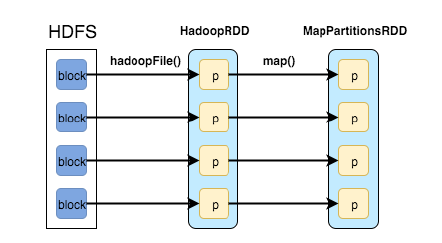
\includegraphics[width=\textwidth]{bilder/Seminartext-img1.png}
\caption{Erstellung RDD aus HDFS \cite{SparkInternals}} 
\end{figure}
Wir haben im vorigen Abschnitt gesehen, wie Spark für die Verteilung das
Partitionieren (Sharding) vornimmt. Neben der Verteilung, die hier wie
im gesamten Projekt durch Scale-Out erfolgt, muss sich Spark auch um
Ausfalltoleranz kümmern. Durch die hohe Anzahl eingesetzter Rechner
steigt die Ausfallwahrscheinlichkeit stark an. Um die Erkennnung
ausgefallener Rechner kümmert sich der Ressourcenmanager und ebenso für
die Inbetriebnahme von Ersatzrechnern bzw. weiterer Rechner für höhere
Leistung.

Spark braucht allerdings einen Mechanismus, wie die Analyse fortgeführt
wird, wenn einer der Rechner ausgefallen ist. Zwei Dinge sind
beantworten: wie kommt man an die lokal gespeicherten Daten? Sie sind durch
den Ausfall nicht mehr zugreifbar und wie wird die Berechnung mit
diesen Daten fortgesetzt?

Die Antwort bei Spark ist erstaunlich einfach. Dies liegt daran, dass
die RDDs immutable sind. Dadurch kann das RDD nach erstmaliger
Fertigstellung nicht in einer unsauberen (dirty) Zustand kommen.
Mechanismen für ein UNDO teilweise fertiger Operationen sind also nicht
notwendig. Stattdessen wird nur ein REDO benötigt. Und um dieses Redo
geht es bei der sogenannten Data Lineage. \ Die Grundidee ist es, für
die RDDs die Herkunft, also die Entstehungsgeschichte aufzuzeichnen
bzw. im Voraus zu berechnen. Zur Erinnerung: das verloren gegangene RDD
ist durch eine Reihe von Transformationen von anderen RDDs aus den
ursprünglichen Eingabedaten entstanden. Fällt nun ein Knoten aus und
geht damit das RDD verloren, so können in der Lineage-Datenstruktur für
dieses RDD die Eltern-RDDs gefunden werden. Sofern diese noch vorliegen
(z.B. auf einem nicht-ausgefallenem Knoten), wird einfach die
aufgezeichnete Operation mit den Eltern-RDDs wiederholt. Sind diese
Eltern-RDDs ebenfalls nicht mehr vorhanden oder ausgefallen, so wird in
der Kette rekursiv durchgegangen. Am Ende stehen die orginalen
Eingabedaten. Das Konzept geht davon aus, dass diese Daten bereits
redundant vorliegen. Das ist auch der Fall, wenn z.B. HDFS genutzt wird
die Originaldaten hiervon geladen werden.

Diese Idee kann nun durch Checkpoints ergänzt werden. Unter einem
Checkpoint versteht man hier eine persistente Kopie von RDDs in einer
tieferen Lineage-Ebene. So muss bei einem Ausfall nur bis maximal zu
diesem RDD in dem Checkpoint zurückgegangen werden. Je länger die
Geschichte eines RDD ist, desto lohnender kann dieser Vorgang sein.
Dagegen spricht natürlich der erhöhte Speicherverbrauch.

Neben der Betrachtung auf RDD-Ebene lässt sich diese Betrachtung auch
auf Partitionsebene innerhalb des RDDs übertragen. Den eigentlich sind
die RDDs ja über mehrere Rechner verteilt (Scale-Out) und auf dem
Rechner liegen dann Partitionen verschiedener RDDs und meist nicht das
ganze RDD.

\section[Programmiermodell]{\selectlanguage{ngerman}\rmfamily
Programmiermodell}
Spark ist sowohl ein Framework, dass einfache Möglichkeiten für
verteilte Analysen bereitstellt, als auch eine Möglichkeit die so
erzeugten Analysen durchzuführen.

In diesem Abschnitt wird nochmal genauer auf das Programmiermodell
eingegangen. Die Daten werden mittels Scale-Out-Algorithmen verteilt
analysiert. Um möglichst hohe Parallelisierung zu erreichen, werden die
Daten in den meisten Fällen als unabhängig angenommen. Beispiele für
Eingabedaten sind Datenbanktabellen oder csv-Dateien.

Die einzelnen Einträge werden unabhängig voneinander vorverarbeitet.
Dies geschieht im Map-Schritt. Dann werden die Ergebnisse
zusammengefügt. Das passiert im Reduce-Schritt. So weit entspricht das
Vorgehen dem MapReduce-Programmiermodell. Spark erweitert es um einige
Operationen.

Dabei werden zwei Typen unterschieden: Aktionen, die aus einem RDD einen
konventionellen Datentyp, wie int, erzeugen. Der andere Typ sind
Transformationen, die aus RDDs wieder andere RDDs erzeugen. Dabei
werden neue RDDs erzeugt und nicht ursprünglichen RDDs verändert, denn
RDDs sind ja immutable.

Man könnte also von einem TransformAction-Programmiermodell als
Weiterentwicklung des MapReduce-Programmiermodells sprechen.

Zu den Transformationen gehören auch filter und flatMap. MapReduce
erweckt den Eindruck, dass es zumindest im Map-Schritt eine
1:1-Abbildung zwischen Elementen des einen RDDs zu Elementen des neuen
RDDs besteht. Natürlich lassen sich auch Elemente entfernen, die dann
im neuen RDD nicht mehr vorkommen (filter) und neue Elemente erzeugen. Dafür
wird eine Liste dieser Elemente als Transformationsergebnis für ein
Element erzeugt und statt map flatmap aufgerufen. Dabei werden alle
Listenelemente zu eigenen Elementen in dem neuen RDD.

Beispiele für Aktionen sind:

\begin{itemize}
\item count()
\item collect()
\item reduce()
\end{itemize}
Beispiele für Transformationen sind:

\begin{itemize}
\item map()
\item filter()
\item flatMap()
\item sample()
\item join()
\item sort()
\end{itemize}
Hinweis: Zur Zeit stellt Spark seine API von RDDs auf Dataframes um.
Diese haben deutlich erweiterte Möglichkeiten. Sie können mit ähnlichen
Operationen wie die von SQL bearbeitet werden.


\subsection{Beispielcode}

Die Beispiele stammen von \url{https://spark.apache.org/examples.html}.

\subsubsection{Bekannte Wordcount}
\lstinputlisting[language=Java]{bilder/wordcount.scala}


\subsubsection{Approximation von PI}
\lstinputlisting[language=Java]{bilder/pi.scala}

Die Funktionsweise ist wie folgt: \ math.random liefert einen Wert
zwischen 0 und 1. Wir stellen uns einen Einheitskreis vor. Sein
Flächeninhalt ist$\pi r^2$, also bei $r=1$ $\pi$. Nun wird geprüft, ob die Koordinate (x,y) in
dem Einheitskreis liegt. Wenn dies der Fall ist, dann wird sie gezählt.
Der Anteil der Koordinaten, die in dem Einheitskreis liegen im
Vergleich zu der Gesamtzahl an Samples, entspricht gerade
$\frac{1}{4}\pi$ Der Faktor Vier
kommt daher, dass wir nur den ersten Quadraten des Einheitskreis
betrachten.

\section[Spark und Distributed Shared
Memory]{\selectlanguage{ngerman}\rmfamily Spark und Distributed Shared
Memory}
Am Anfang haben wir als ein Ziel von Spark die Abstraktion für
Distributed Shared Memory beschrieben. Das wollen wir nun nochmal
aufgreifen und beide vergleichen. Dadurch, dass die Operationen
gegenüber der Distributed Shared Memory eingeschränkt werden, nämlich
insbesondere Veränderungen nur bei gleichzeitiger Kopie des RDDs
vorgenommen werden können, entfallen viele Aufgaben. Distributed Shared
Memory funktioniert wie verteilter Arbeitsspeicher, d.h. die einzelnen
Rechner können mehr oder weniger unreguliert Lese- und
Schreiboperationen vornehmen. Damit das nicht im Chaos endet, müssen
sie sich Protokolle zur Synchronisation nutzen. 

Betrachten wir einige Aufgaben genauer:


\begin{itemize}
\item Konsistenz der Daten sicherstellen
\end{itemize}
Ist bei RDDs nicht notwendig, da die RDDs immutable sind. Es muss nur
überwacht werden, ob das RDD vollständig erzeugt wurde. Dadurch wird der
ganze Transformationsvorgang atomar. Bei Distributed Shared Memory ist
das nicht so. Da sind zusammengehörige Schreiboperationen nicht atomar,
d.h. es ist durchaus möglich, dass der erste Teil der
Schreiboperationen bereits umgesetzt wurde (z.B. Kontostand bei einer
Überweisung verringern), der zweite Teil aber nicht (z.B. Kontostand
beim Empfänger erhöhen). Deshalb muss die Anwendung hier ein spezielles
Protokoll zwischen den Knoten einführen.

\begin{itemize}
\item Fault Recovery
\end{itemize}
Kann bei RDDs durch Lineage vergleichsweise einfach vorgenommen werden.
Bei Distributed Shared Memory ist wieder ein kompliziertes Protokoll
notwendig. Checkpoints sichern die Daten. Da die Konsistenz aber nicht
notwendigerweise gegeben ist, braucht es Rollback-Vorgänge. 

Eindeutiger Nachteil der RDDs ist ihr schlechter Umgang mit
feingranualaren Schreibevorgänge, d.h wenn nur wenige Elemente eines
RDDs geändert werden sollen. Distributed Shared Memory liegt hier
eindeutig vorne, da alle Operationen feingranular erfolgen können.

\section[Spark{}-Architektur]{\selectlanguage{ngerman}\rmfamily
Spark-Architektur}
Hauptaugenmerk in diesem Abschnitt soll auf der Berechnung der Job
Stages liegen \cite{SparkInternals}. Mit Hilfe der Transformationen und Aktionen lassen sich
komplexe Abfolgen von Operationen auf unterschiedlichen RDDs und auch
in Kombination dieser RDDs erzeugen. Während die Transformationen für
alle Partitionen parallel ausgeführt werden können, müssen die parallel
erfolgenden Operationen durch Spark erst berechnet werden.

Dazu werden die komplexen Operationsfolgen in Stages unterteilt. Sie
entsprechen den Knoten in einem DAG (einem azyklischen Graphen).
Dadurch entsteht eine partielle Ordnung der Stages. Stehen zwei Stages
weder in einer Vor- noch in einer Nacheinander-Beziehung, so können sie
parallel berechnet werden, sofern ihre Eltern-RDDs bereits berechnet
wurden. 

Ein entscheidender Unterschied stellen hier die Operationen da. Sind die
Operationen Joins oder groupByKey, so müssen alle daran beteiligten
RDDs vollständig berechnet sein, damit die Operation ausgeführt werden
kann. Man spricht dann von einer wide dependency. D.h. bei der
Ausführung muss das erste RDD auf die anderen RDDs warten. Andere
Operation wie map, union, join mit co-partitionierten Input oder filter
brauchen das nicht. Sie liegen innerhalb eines Stages in einer Abfolge.
Man spricht hier von narrow dependencies.

\begin{figure}
\centering
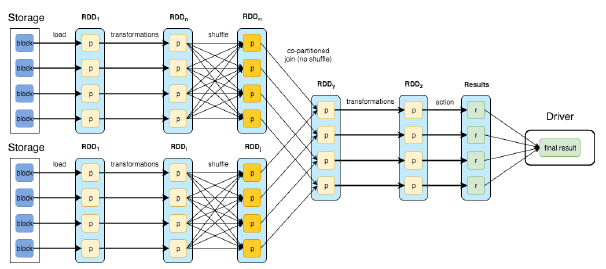
\includegraphics[width=\textwidth]{bilder/Seminartext-img2.png}
\caption{Spark Stages \cite{SparkInternals}}
\end{figure}

\bigskip

\subsection[Durchlauf durch
Komponenten]{\selectlanguage{ngerman}\rmfamily Durchlauf durch
Komponenten}
Betrachten wir nun Einbindung der Job-Stage-Berechnung in die
Architektur. Alles fängt mit den RDDs an, die inkl. ihrer Lineage aus
dem Javacode ermittelt werden. Sie werden als DAG in den DAGScheduler
eingegeben. Dieser berechnet die möglichen Jobstages und ermittelt
daraus TaskSets für die einzelnen Rechnenknoten. Er gibt sie an den
Clustermanager weiter. Dieser verteilt sie dann an geeignete Knoten. In
diesen Knoten, den Executors, werden diese dann in Threads ausgeführt. 

\begin{figure}
\centering
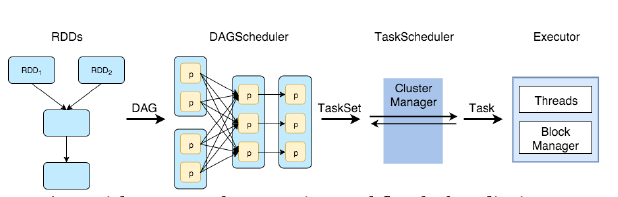
\includegraphics[width=\textwidth]{bilder/Seminartext-img3.png}
\caption{Spark Architektur \cite{SparkInternals}}
\end{figure}

\bigskip

\section[Vor{}- und Nachteile von
Spark]{\selectlanguage{ngerman}\rmfamily Vor- und Nachteile von Spark}
Fassen wir nochmal die Vorteile und Nachteile von Spark zusammen.
Entscheidend ist die Art von Programm, das ausgeführt werden soll.
Jenachdem ist Spark besser oder weniger gut geeignet.

Schlecht geeignete Programme sind Programme mit vielen asynchronen,
feingranularen Updates auf einem gemeinsamen Zustand. Dies würde zu
einer Explosion der Anzahl von RDDs führen. Beispiele hierfür sind
Web-Anwendungen und inkrementelle Web-Crawler. Alternativen wären
RAMCloud, Percolator und Piccolo.

Gut geeignete Programme führen Bulk Writes auf vielen Daten aus.
Insbesondere dann, wenn Datenlokalität ausgenutzt werden kann, ist
Spark gut geeignet. Spark punktet dann mit effizienter Fault Tolerance
durch Lineage und Ausgleich von langsamen Knoten, da kein Rollback
notwendig ist.

\section[Funktionsweise Spark
Streaming]{\selectlanguage{ngerman}\rmfamily Funktionsweise Spark
Streaming}
Als letztes wollen wir noch die Funktionsweise einer Variante von Spark
anschauen, nämlich Spark Streaming. Spark Streaming wird in \cite{SparkStreaming} beschrieben.
 Wenn man nicht auf periodisch
ausgeführte Analysen warten möchte, sondern gewissermaßen live auf
Ergebnisse zugreifen möchte, kann Spark Streaming eingesetzt werden.

Die Eingabedaten kommen dabei als kontinuierlicher Stream. Sie werden in
Microbatches zerlegt, d.h. es werden z.B. die Daten einer Sekunde
zwischengespeichert. Dann wird ein herkömmlicher Spark-Job auf dem
Batch ausgeführt. Dies wird kontinuierlich für die einkommenden Streams
gemacht. Spark nennt dieses Vorgehen D-Streams. Es ist ein Denkmodell
dafür, dass einkommende Einträge als Microbatches in einem RDD
gespeichert werden. Auf diesem werden dann parallel deterministische
Operationen ausgeführt, analog wie bei der Batch-Analyse. Ein D-Stream
ist also eine Folge von Datensets. Es ist keine komplexe
Synchronisation der einzelnen Knoten notwendig. Sie operieren
unabhängig voneinander und bekommen ihre Aufgaben aus dem DAGScheduler
vorgegeben. Sie greifen nicht auf gemeinsamen Speicher schreibend zu.
\ Ausfälle von Knoten sowie zu langsame Knoten lassen sich genau wie
sonst auch beheben. 

\begin{figure}
\centering
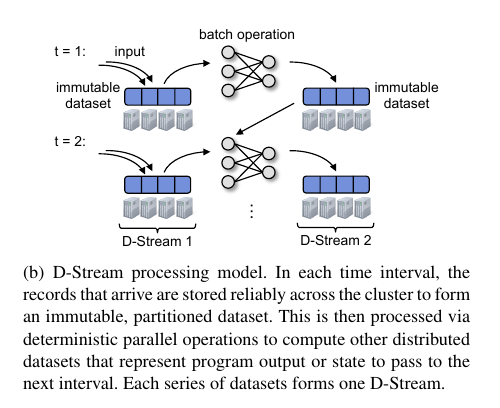
\includegraphics[width=\textwidth]{bilder/Seminartext-img4.png}
\caption{Sparks DStreams \cite{SparkStreaming}}
\end{figure}
\subsection[alternatives, nicht verwendetes
Denkmodell]{\selectlanguage{ngerman}\rmfamily alternatives, nicht
verwendetes Denkmodell}
Ein alternatives Modell wäre der Continuous Operator. Dabei haben die
Nodes einen inneren Zustand, ggfs. gibt es einen dezidierten
gemeinsamen Zustand. Ausfalltoleranz kann dann mit einem
Synchronisationsprotokoll erreicht werden, das Replikation vorsieht.
Schwieriger ist hier die Recovery. Da die zusammenhängenden
Schreiboperationen nicht atomar ausgeführt werden, braucht man wie bei
bei Distributed Shared Memory Rollback und weitere Mechansimen.

Allerdings können hiermit auch komplexere Berechnungen vorgenommen
werden. Es gibt die künstlichen Microbatches-Grenzen nicht.
Dementsprechend sind z.B. Rolling-Windows einfacher. 